\documentclass[12pt, a4paper]{article}

\voffset=-1.5cm
\oddsidemargin=0.0cm
\textwidth = 470pt

\usepackage{epsfig}
\usepackage{subfigure}
%\usepackage{amscd}
\usepackage{amssymb}
\usepackage{amsbsy}
\usepackage{amsthm}
%\usepackage[dvips]{graphicx}
\usepackage{natbib}
\usepackage{framed}
\bibliographystyle{chicago}



\begin{document}
	\author{Kevin O'Brien}
	\title{MA4128}
	
%	\tableofcontents \setcounter{tocdepth}{2}
\subsection*{Interpreting $p-$values}

For the purposes of this module, we will use the following rules of thumb.
If we do not have a significant $p-$value, we fail to reject the null hypothesis.
If we have a significant result, we reject the Null Hypothesis.
\begin{itemize}
	\item p-value is greater than 0.05 - Not Significant
	\item p-value is between 0.05 and 0.01 - Significant
	\item p-value is between 0.01 and 0.001 - Very Significant
	\item p-value is less than 0.001 - Highly Significant
\end{itemize}
Outside of this module, you are advised to research the proper use, and the amount of misuse, of p-values in scientific research

\bigskip

\noindent \textbf{Example 1  - Significant Result}
\begin{figure}[h!]
\centering
\includegraphics[width=0.8\linewidth]{grubbsTest}
\caption{}
\label{fig:gruubsTest}
\end{figure}

\bigskip
\noindent \textbf{Example 2 - Result Not Significant}
\begin{figure}[h!]
\centering
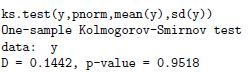
\includegraphics[width=0.55\linewidth]{kstest}
\caption{}
\label{fig:kstest}
\end{figure}


\end{document}